\documentclass[11pt,a4paper]{article}
\usepackage{a4wide}
\usepackage{english}

\usepackage[left=2cm,right=2cm,top=1.5cm,bottom=1.5cm]{geometry}
\usepackage[utf8]{inputenc} 
\usepackage{lmodern}
\usepackage{pifont}
\usepackage{epsdice}
\usepackage{epsfig}
\usepackage{epstopdf} 
\usepackage{amsmath,amssymb,amsfonts}
\usepackage{subcaption}
\usepackage{array}
\usepackage{makecell}
\usepackage{graphicx}
\usepackage{xargs}
\usepackage{float}
\usepackage{mathtools}
\usepackage{subcaption}
\usepackage{amsmath}
\usepackage{xcolor}
\usepackage{multirow}
\usepackage{float}
\usepackage[italic]{hepnames}
%https://www.sys.kth.se/docs/texlive/texmf-dist/doc/latex/hepnames/hepnames.pdf%

\pagenumbering{arabic}


\setlength{\parindent}{0pt}
%--------------------------------------------------
\title{Data cleaning for \PKshort decay reconstruction ML model CBM}
\author{Julian Nowak}
\date{VIII 2021}
%-------------------------------------------------------------
\begin{document}

\maketitle
%------------------------reconstruction
\section{\PKshort (short lived Kaon) reconstruction:}
\noindent\begin{minipage}{0.6\textwidth}
K-short (short lived Kaon) reconstruction:
\begin{itemize}
    \item Mother particle: \PKshort (PDG = 310)
    \item Mass: 497.611±0.013 MeV/$c^2$
    \item Mean lifetime: $8.958\cdot 10^{-11}$ s
    \item Charge = 0
    \item Meson, composed of two quarks: \Pdown\APstrange or \Pstrange\APdown
    \item Strange particle
\end{itemize}
\end{minipage}
\noindent\begin{minipage}{0.4\textwidth}
    \centering
    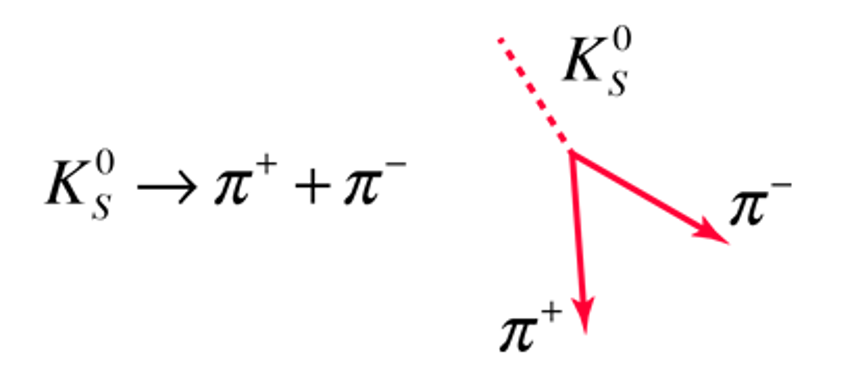
\includegraphics[width=\textwidth]{images/kdecay1.png}
    \PKshort decay diagram \cite{kdecay1}
\end{minipage}
\\\\
In the main decay mode:
\begin{figure}[H]
    \centering
    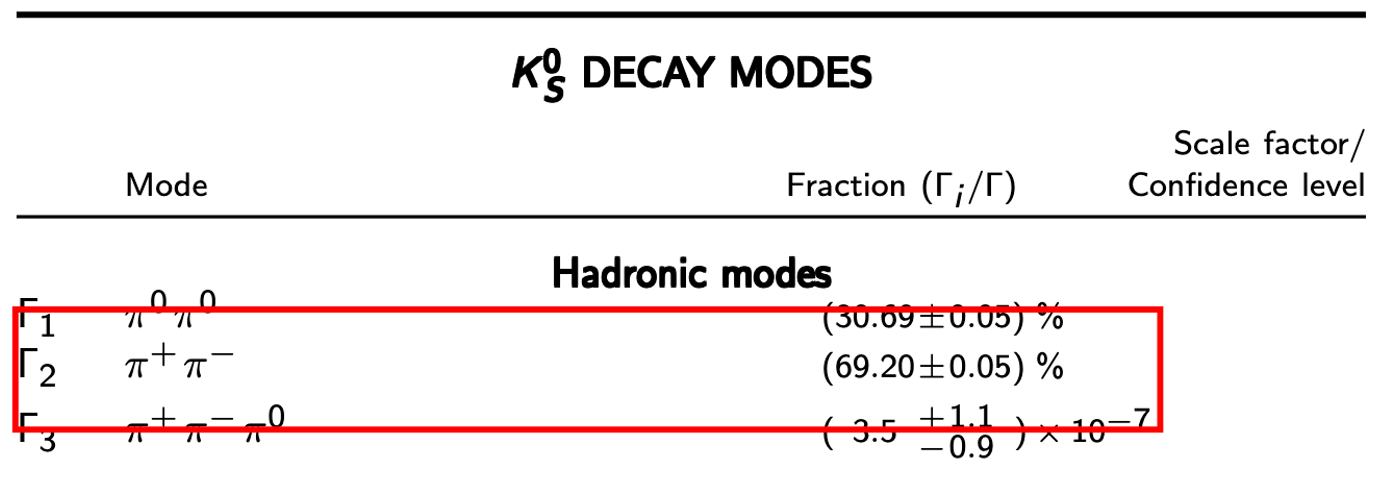
\includegraphics[width=.8\textwidth]{images/kdecay2.png}
    \caption{\PKshort decay modes \cite{kdecay2}}
    \label{fig:my_label}
\end{figure}

\PKshort particle decays into \Pgpp (PDG = 211) and \Pgpm (PDG = -211). Mass of each pion equals 139.57039(18) MeV/$c^2$

\newpage
%----------------------- objective
\section{Objective}
Our model will be trained to correctly distinguish between the \emph{signal} - pairs of \Pgpp and \Pgpm which where produced in the \KPshort decay, and \emph{background} - pairs of pions which aren't result of the \KPshort decay. We assume that the majority of the particles of invariant mass in $5 \sigma$ region around the \KPshort mass peak should be recognized as the K-short candidates. The ML model learns, which parameters values should be associated with the signal, and which with the background. As the mathematical ML model has no clue which data values are physically correct, we need to clean the data.
%---------------------- data cleaning
\section{Data cleaning}
To reject the numeric values of parameters which don't have physical sens, but are present in the data set, we apply some cuts before the beginning of the model training. Similarly, we reject some values which might be possible, but are rare enough, so we reject them to reduce the data.

%----------------------- Invariant mass
\subsection{Invariant mass}
As the K-short particle decays into two pions (in the decay mode we're able to reconstruct) its invariant mass cannot be smaller than the mass of the two pions, so:
\begin{center}
    mass $>$ 0.279 GeV/$c^2$
\end{center}
Also, to reduce the amount of data, we only accept the particles with:
\begin{center}
    mass $<$ 2.0 GeV/$c^2$
\end{center}

%---------------- distances
\subsection{Distances and \emph{x, y, z} cordinates}
Distance between the primary and the secondary vortex $l$ and the distance of closest approach between the two pions $DCA$ obviously cannot be smaller than 0. So:
\begin{center}
    $DCA$, $l$, $\frac{l}{\Delta l}$ $> 0$
\end{center}
Also, due to the sizes of the tracking system (the largest station has an are of 100 cm$^2$):
\begin{center}
    $DCA < 100 $ cm
\end{center}
For the same reason:
\begin{center}
    $|x|, |y| < 50$ cm
\end{center}
As the particle has to hit 3 stations of the tracking system, and the last two are placed above 80cm"
\begin{center}
    $l < 80$cm
\end{center}
For the same reason:
\begin{center}
    $|z| < 80$ cm
\end{center}
To reduce the data:
\begin{center}
    $\frac{l}{\Delta l} < 5000$
\end{center}
%----------------- momentums
\subsection{Momentums}
The fixed target geometry of the detector requires that:
\begin{center}
    $p_Z > 0 $ GeV/c
\end{center}
To reduce the data, we only preserve:
\begin{center}
    $p < 20$ Gev/c; $p_T < 3$ GeV/c
\end{center}
%-------------- chi square
\subsection{Chi square}
Following simple algebra, all chi square values must be bigger than zero:
\begin{center}
    $\chi^2 > 0$
\end{center}
Following the work of Olga for \PLambda decays, for now I set the rest of chi square cut values to:
\begin{itemize}
    \item $\chi^2$ first and second $< 3 \cdot 10^7$
    \item $\chi^2_{geo} < 1000$
    \item $\chi^2_{topo} < 100000$
\end{itemize}

%----------------------- pseudorapidity
\subsection{Pseudorapidity}
As pseudorapidity $\eta = -\ln{\tan(\frac{\theta}{2})}$, and the Silicon Tracking System (STS) cover the polar angles between 2.5$^{\circ}$ and 25$^{\circ}$, we decide to constrain the pseudorapidity values:
\begin{center}
    $ 1< \eta < 4 $
\end{center}

%------------------ bibliography
\begin{thebibliography}{9}

\bibitem{kdecay1} 
\url{http://hyperphysics.phy-astr.gsu.edu/hbase/Particles/kaon.html}

\bibitem{kdecay2}
\url{https://pdg.lbl.gov/2021/listings/contents\_listings.html}


\end{thebibliography}

\end{document}